\chapter{Introduction} \label{chap:intro}

\section{Controllers and their specifications}

\subsection{ESP32 Micro-controller}

\begin{figure}[h!]
\centering
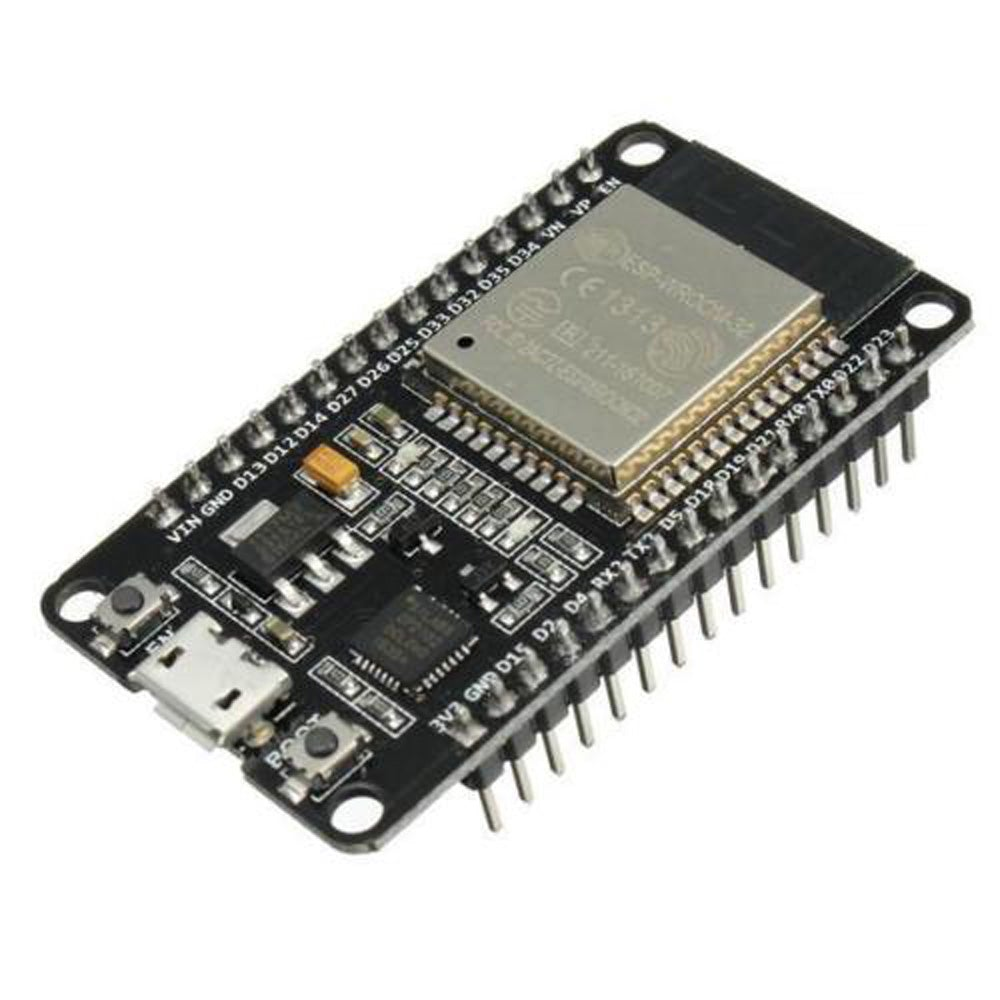
\includegraphics[width=5cm]{./Figures/ESP32.jpg}
\caption{ESP-WROOM-32 Dev Kit}
\label{ESP32}
\end{figure}

ESP32 is among the popular micro-controllers. The ESP32 series utilizes Tensilica's Xtensa LX6 microprocessor. ESP32 integrates an antenna switch, RF balun, power amplifier, low-noise receive amplifier, filters,
and power management modules. Unlike Arduino Uno it provide on-board WiFi and Bluetooth functionalities. It supports various interfaces such as  UART, I2C, SPI, PWM module, GPIO, ADC/DAC, SD card, etc. It operates on voltage supply of 3-3.6V. It is a successor to the ESP8266 micro-controller.~\cite{esp32}

\subsection{Vaman Pygmy BB4} 
\par Vaman is a development board based around the Pygmy Stamp module, and brings on-board WiFi/BT/BLE connectivity with ESP32, as well as an 18650 battery option, $\mu$SD Card (connected to ESP32), possibility to use EOSS3 in smartphone mode with the ESP32 as the Host, and all EOSS3 pins accessible. A BMX160 provides an AMG IMU, supplemented by a BNO055 smart fusion sensor. A DPS310 provides Pressure, Humidity and Temperature monitoring.~\cite{Vaman}

\begin{figure}[h!]
\centering
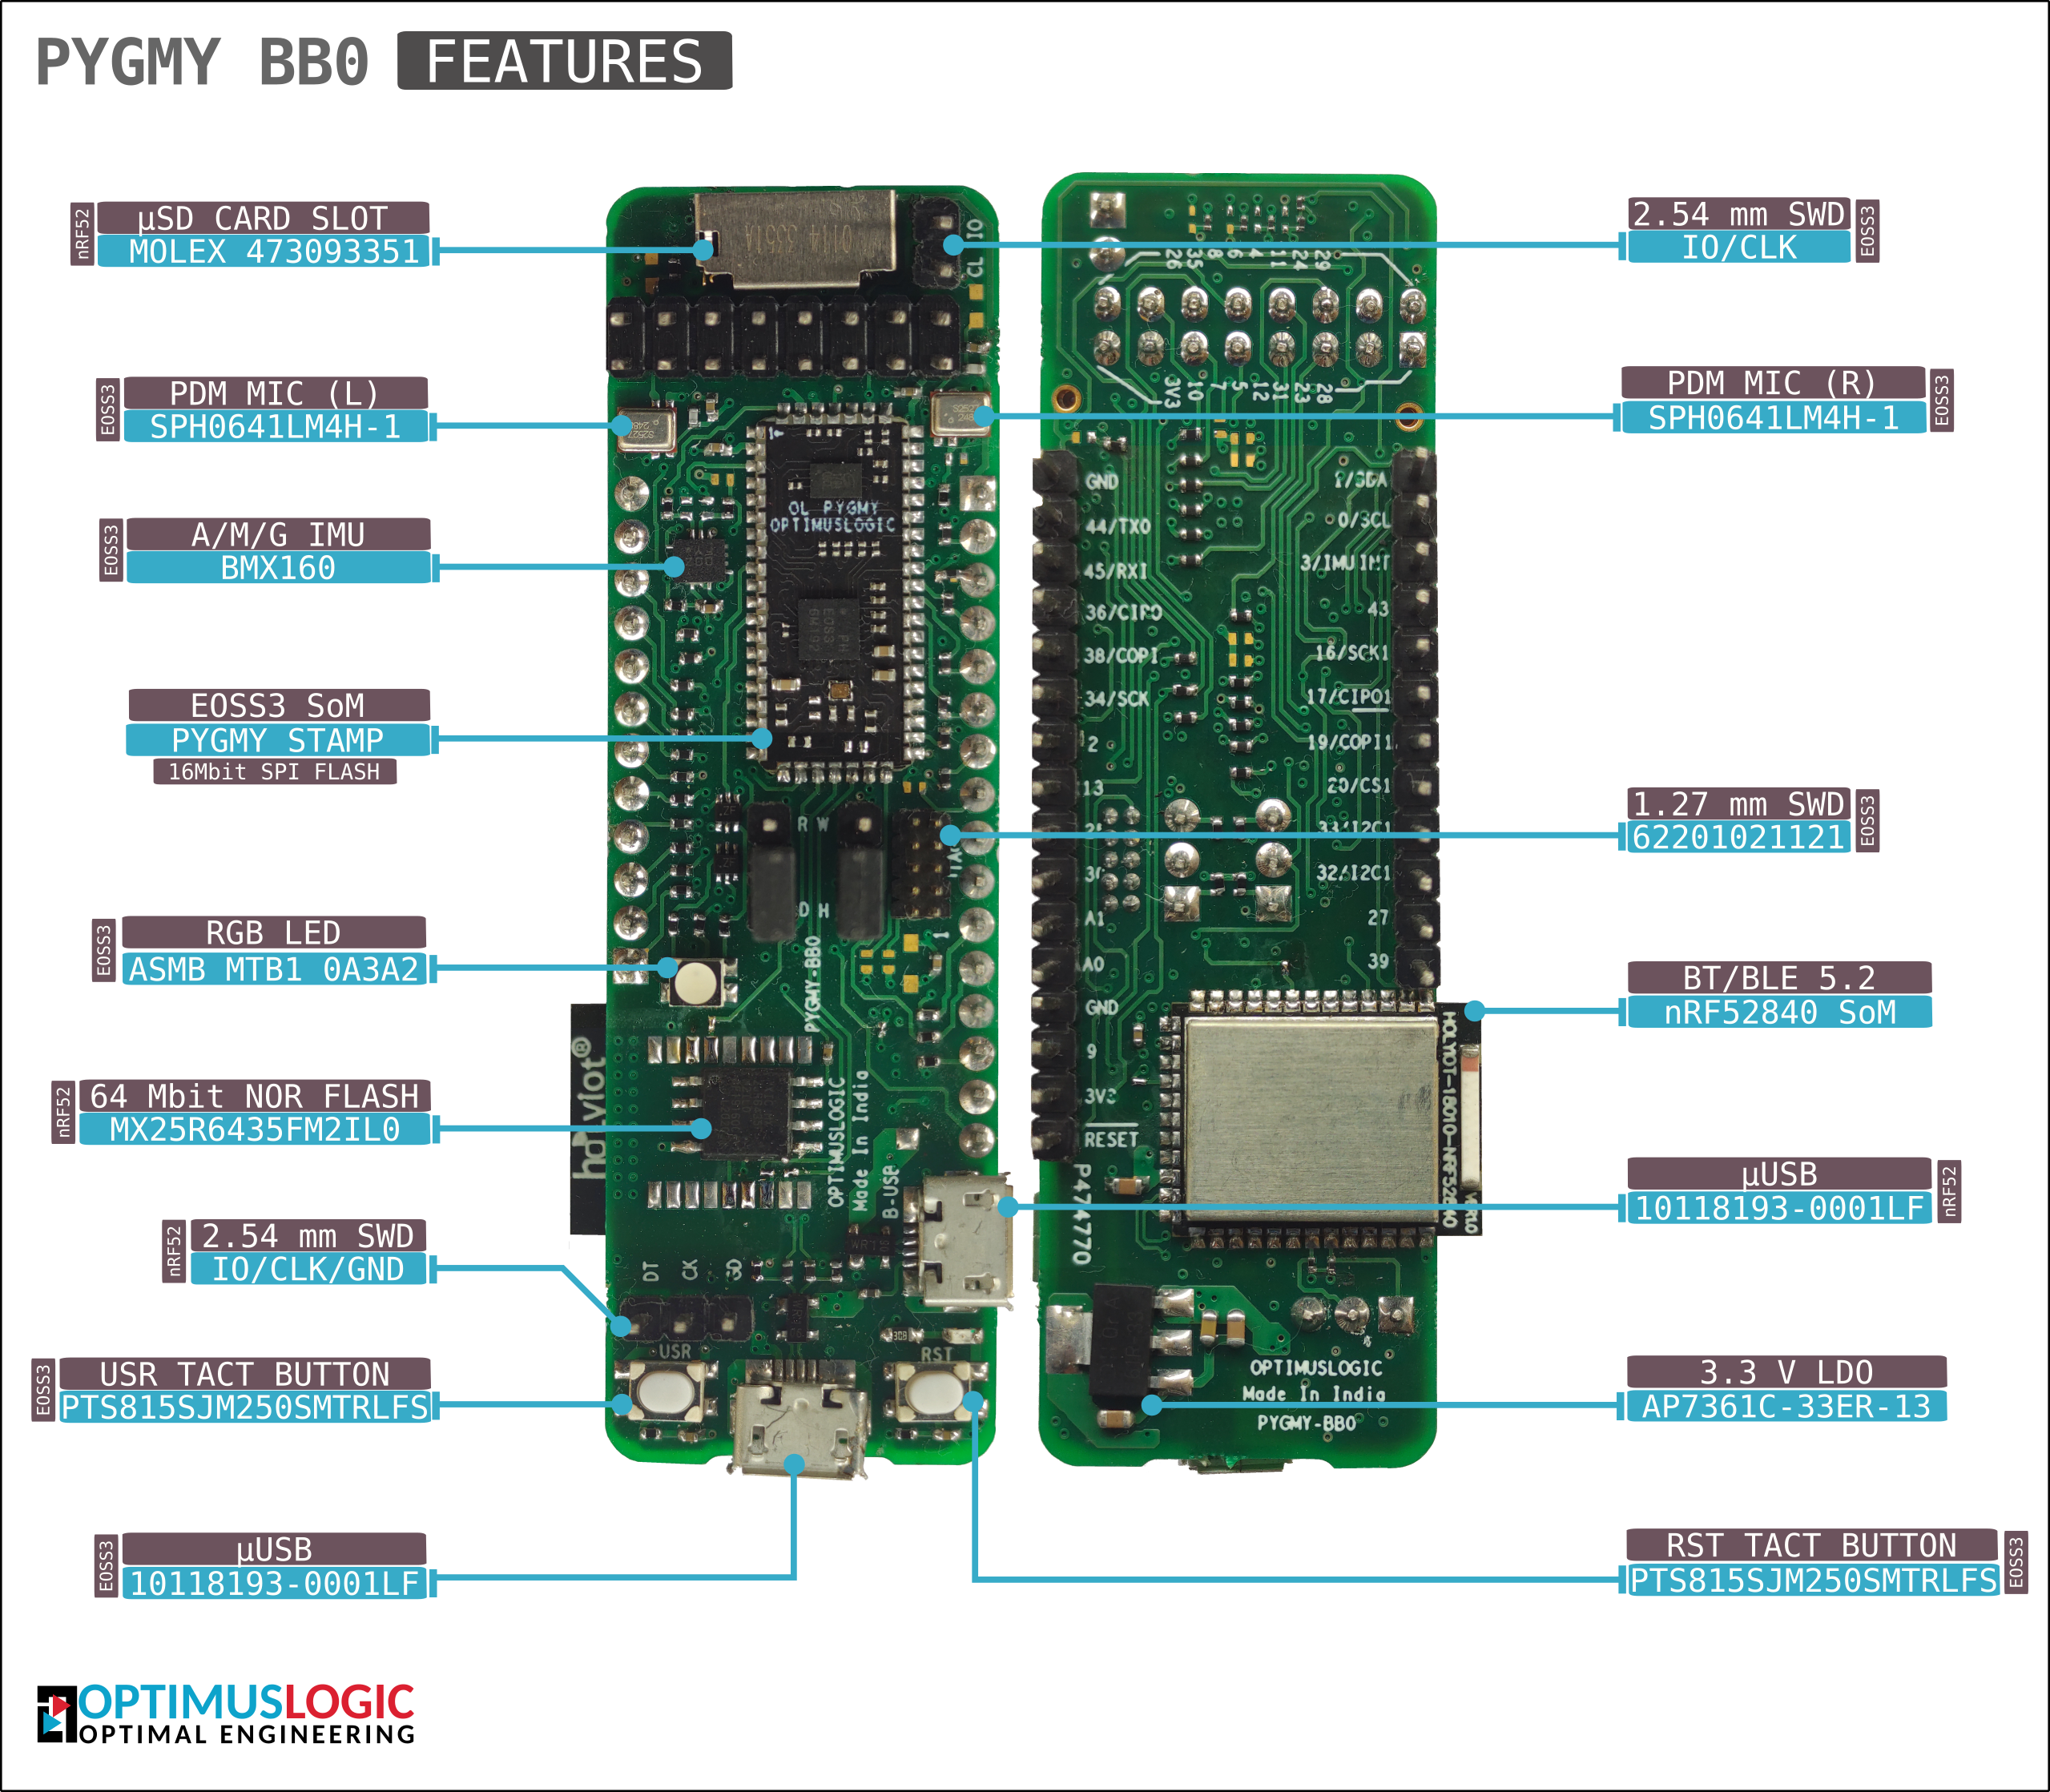
\includegraphics[width=14cm]{./Figures/Vaman.png}
\caption{Vaman (Pygmy BB4)}
\label{vaman}
\end{figure}

\subsection{Arduino Uno}  

\par Arduino is an open-source development board ideal for handling a variety of applications. It is inexpensive as well as feature-packed. It is compatible with a variety of daughter boards that can be attached to it.  The low-power Bluetooth shield, along with the Wi-Fi and Ethernet shields, allows increased communication functionalities. 

\begin{figure}[h!]
\centering
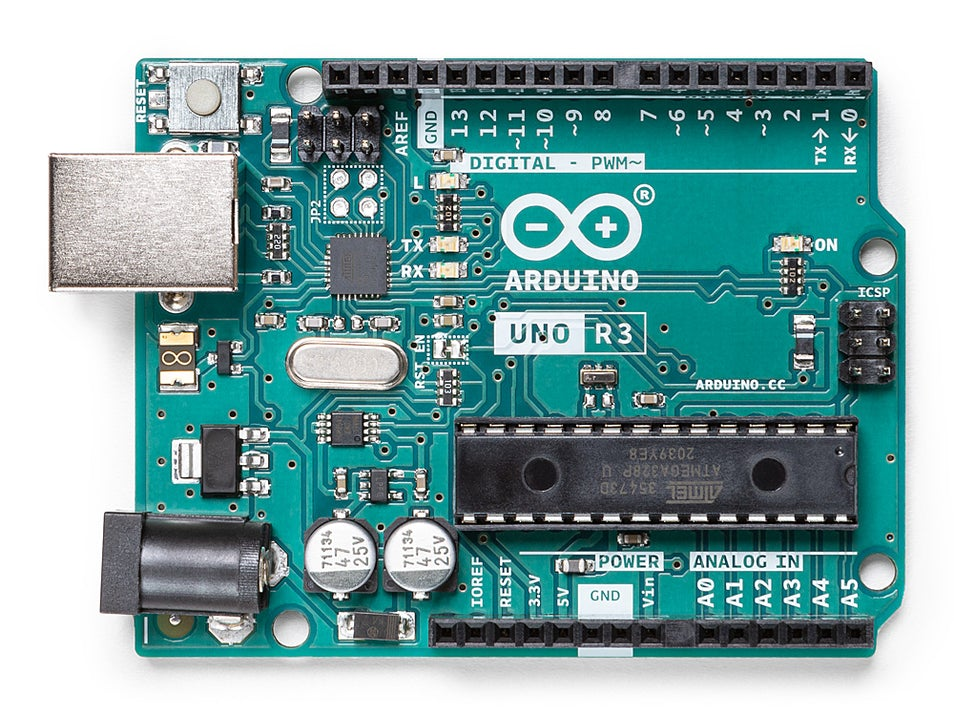
\includegraphics[width=6cm]{./Figures/Arduino_Uno.jpg}
\caption{Arduino Uno R3}
\label{Arduino_Uno_R3}
\end{figure}

\subsection{Raspberry Pi 3B}

\begin{figure}[h!]
\centering
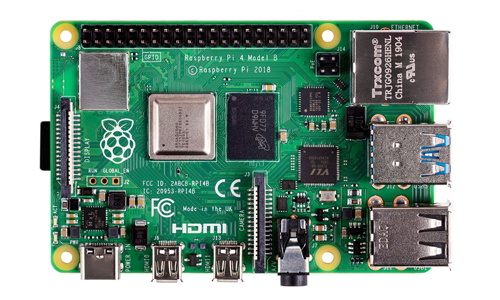
\includegraphics[width=9cm]{./Figures/Rpi_3B.png}
\caption{Raspberry Pi 3B}
\label{Rpi_3B}
\end{figure}

\par Raspberry Pi (RPi) is an on-board computer and it is among the most popular development boards. The Raspberry Pi runs a customized version of Linux called Raspberry Pi OS. It has all the features of a personal computer. This board has USB interfaces that allow it to connect to peripherals (such as a mouse and keyboard), USB storage, etc. HDMI interface can be used to connect displays to the board having up to 4K resolution. Additionally, it has other ports/interfaces, including USB-C (power), a 2-lane MIPI CSI port (camera), a 3.5mm audio jack (audio), and RJ-45 (Ethernet). WiFi and Bluetooth 5.0 support are provided by the Raspberry Pi.

\begin{table}[H]
\centering
\begin{tabular}{|l|c|c|c|}
\hline
\textbf{Parameters} & \textbf{Arduino Uno} & \textbf{Raspberry Pi 3B} & \textbf{ESP-32} \\ \hline
\textbf{Processor} & ATMega328P & \begin{tabular}[c]{@{}c@{}}Quad-core Broadcom \\ BCM2837 (4×Cortex-A53)\end{tabular} & \begin{tabular}[c]{@{}c@{}}Xtensa Dual-Core 32-bit \\ LX6 with 600 DMIPS\end{tabular} \\ \hline
\textbf{GPU} & - & \begin{tabular}[c]{@{}c@{}}Broadcom VideoCore IV \\ @ 250 MHz\end{tabular} & - \\ \hline
\textbf{Operating voltage} & 5V & 5V & 3.3V \\ \hline
\textbf{Clock speed} & 16 MHz & 1.2GHz & 26 MHz – 52 MHz \\ \hline
\textbf{System memory} & 2kB & 1 GB & \textless{}45kB \\ \hline
\textbf{Flash memory} & 32 kB & - & up to 128MB \\ \hline
\textbf{EEPROM} & 1 kB & - & - \\ \hline
\textbf{\begin{tabular}[c]{@{}l@{}}Communication \\ supported\end{tabular}} & \begin{tabular}[c]{@{}c@{}}IEEE 802.11 b/g/n\\ Bluetooth via Shield\end{tabular} & \begin{tabular}[c]{@{}c@{}}IEEE 802.11 b/g/n\\ Bluetooth, Ethernet Serial\end{tabular} & IEEE 802.11 b/g/n \\ \hline
\textbf{\begin{tabular}[c]{@{}l@{}}Development \\ environments\end{tabular}} & Arduino IDE & \begin{tabular}[c]{@{}c@{}}Any linux \\ compatible IDE\end{tabular} & Arduino IDE, Lua Loader \\ \hline
\textbf{\begin{tabular}[c]{@{}l@{}}Programming \\ language\end{tabular}} & Embedded C, C++ & \begin{tabular}[c]{@{}c@{}}Python, C, C++, Java,\\ Scratch, Ruby\end{tabular} & Embedded C, C++ \\ \hline
\textbf{I/O Connectivity} & SPI I2C UART GPIO & \begin{tabular}[c]{@{}c@{}}SPI DSI UART \\ SDIOCSI GPIO\end{tabular} & UART, GPIO \\ \hline
\end{tabular}
\caption{Comparison between Arduino Uno, Raspberry Pi 3B and ESP-32~\cite{Comparision_controllers}}
\end{table}

